\documentclass[a4paper,12pt]{article}

\usepackage{graphicx}
\usepackage{caption}
\usepackage{subcaption}
\usepackage{tikz}
\usepackage{pgf}
\usepackage{amsmath}
\usepackage{amssymb}
\usetikzlibrary{arrows.meta}
\usepackage[utf8]{inputenc}
\usepackage[english,greek]{babel}
\usepackage{hyperref}

\title{Προσομοίωση και Μοντελοποίηση \newline Δυναμικών Συστημάτων \newline 
\selectlanguage{english}Project\selectlanguage{greek}}
\author{Ρουσομάνης Γεώργιος (ΑΕΜ: 10703)}
\date{Ιούνιος 2025}

\begin{document}

\maketitle

\section*{Εισαγωγή}

\section*{Θέμα 1}

Σε αυτό το μέρος μελετάται ένα γραμμικό δυναμικό σύστημα δεύτερης τάξης της μορφής:
\begin{equation}
\dot{x}(t) = A x(t) + B u(t),
\end{equation}
όπου $x(t) \in \mathbb{R}^2$ είναι το διάνυσμα των καταστάσεων, και $u(t) \in \mathbb{R}$ 
η είσοδος του συστήματος. Οι πίνακες $A \in \mathbb{R}^{2 \times 2}$ και 
$B \in \mathbb{R}^{2 \times 1}$ είναι άγνωστοι αλλά σταθεροί. Επίσης, γνωρίζουμε ότι:
\begin{equation}
-3 \leq a_{11} \leq -1, \quad \quad b_2 \geq 1.
\label{eq:restrictions}
\end{equation}

Σκοπός είναι η ανάπτυξη και ανάλυση ενός αλγορίθμου πραγματικού χρόνου για την εκτίμηση  
$\hat{A},\,\hat{B}$ των πινάκων $A$ και $B$, με δεδομένο ότι τόσο η είσοδος $u(t)$ όσο και  
οι καταστάσεις $x(t)$ είναι μετρήσιμες. Για τη σχεδίαση του αλγορίθμου, αρχικά υποθέτουμε ότι  
δεν υπάρχουν διαταραχές στις μετρήσεις των καταστάσεων του συστήματος. Στη συνέχεια,  
εισάγεται στο σύστημα σφάλμα πόλωσης και επανασχεδιάζεται ο αλγόριθμος, με στόχο  
τη μελέτη της επίδρασης του σφάλματος στην ακρίβεια των εκτιμήσεων. Για σκοπούς προσομοίωσης,  
χρησιμοποιούνται ως πραγματικές τιμές οι παρακάτω πίνακες:
\[
A = 
\begin{bmatrix}
-2.15 & 0.25 \\
-0.75 & -2
\end{bmatrix}, \quad
B = 
\begin{bmatrix}
0 \\
1.5
\end{bmatrix}.
\]

\subsection*{Εκτίμηση Παραμέτρων χωρίς Σφάλμα Πόλωσης}

Πρωτού προχωρήσουμε στη σχεδίαση του αλγορίθμου πραγματικού χρόνου για την εκτίμηση των $A,\,B$,  
πρέπει να επιλέξουμε το είδος της εισόδου που θα εφαρμόσουμε στο σύστημα, καθώς και τη συχνότητα  
δειγματοληψίας. Μία συνήθης πρακτική για την επιλογή της συχνότητας δειγματοληψίας είναι να την  
ορίζουμε περίπου δέκα φορές μεγαλύτερη από το εύρος ζώνης του συστήματος. Ωστόσο, επειδή το μοντέλο  
μας υπάγεται στην κατηγορία ``γκρι κουτί'', η εκ των προτέρων γνώση μας για το σύστημα δεν επαρκεί  
για τον άμεσο υπολογισμό του εύρους ζώνης.

\subsubsection*{Επιλογή Συχνότητας Δειγματολειψίας}

Εφαρμόζουμε βηματική είσοδο στο σύστημα ώστε να εκτιμήσουμε την κυρίαρχη σταθερά χρόνου  
και να αποκτήσουμε μία πρώτη εικόνα για τη δυναμική του. Η βηματική απόκριση του συστήματος  
παρουσιάζεται στο Σχήμα~\ref{fig:task1_step_response} για συχνότητα δειγματοληψίας $f_s = 1$
\selectlanguage{english}kHz\selectlanguage{greek}. Η $f_s$ επιλέχθηκε αυθαίρετα ως μία υψηλή τιμή, 
επαρκής για να αποτυπώσει επαρκώς τη δυναμική του συστήματος.

Από το σχήμα είναι εμφανές ότι η απόκριση της κατάστασης $x_2(t)$ είναι ταχύτερη αυτής της $x_1(t)$,
συνεπώς η σταθερά χρόνου του συστήματος θα προσδιοριστεί μέσω της $x_2(t)$. Στην απόκριση της
$x_2(t)$ δεν παρατηρείται υπερύψωση, άρα ο χρόνος αποκατάστασης $t_s$ ορίζεται ως ο χρόνος που απαιτείται
ώστε το σύστημα να φτάσει στο $98\%$ της εξόδου του. Από το σχήμα βλέπουμε ότι $t_s \approx 2$
\selectlanguage{english}sec\selectlanguage{greek}. Η σταθερά χρόνου είναι $\tau \approx t_s / 4 = 0.5$
\selectlanguage{english}sec\selectlanguage{greek}. Συνεπώς, η συχνότητα δειγματολειψίας πρέπει να 
ικανοποιεί $f_s > 10 / \tau = 20$\selectlanguage{english}Hz\selectlanguage{greek}.

Για το πραγματικό σύστημα, οι ιδιοτιμές του πίνακα $A$ είναι $\lambda_{1,2} = -2.075 \pm 0.4265j$, 
και η σταθερά χρόνου $\tau = \frac{1}{\zeta \omega_n} = 0.482$, η οποία είναι πολύ κοντά στην αρχική 
μας εκτίμηση.

\begin{figure}
    \centering
    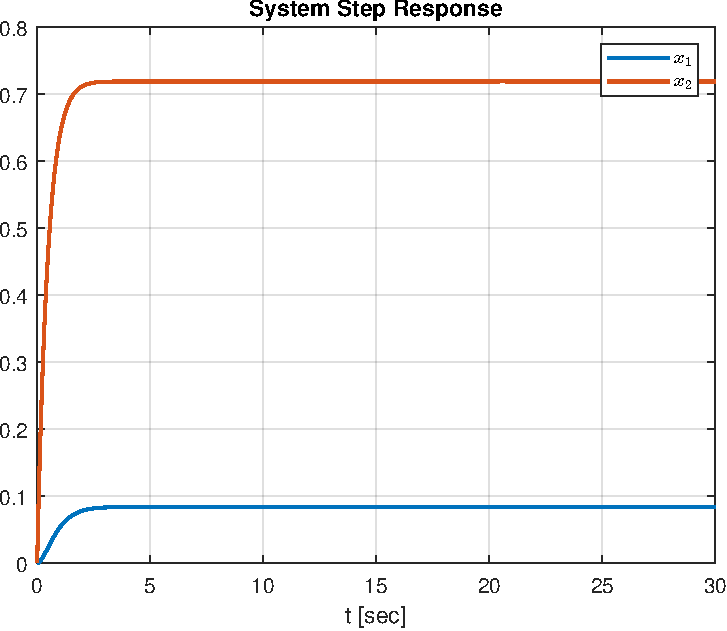
\includegraphics[width=0.75\linewidth]{plot/task1_step_response.pdf}
    \caption{Βηματική απόκριση του συστήματος}
    \label{fig:task1_step_response}
\end{figure}

\subsubsection*{Επιλογή Εισόδου}

Για να αποτυπωθεί πλήρως η δυναμική του συστήματος, είναι σημαντικό η είσοδος να περιέχει αρκετές
συχνότητες ώστε να διεγείρει όλους τους ρυθμούς του συστήματος. Επίσης, με κατάλληλη επιλογή της
εισόδου ώστε να ικανοποιεί την Συνθήκη Εναπομείνουσας Διέγερσης (ΣΕΔ), οι μέδοδοι εκτίμησης παραμέτρων 
πραγματικού χρόνου (κλίσης, \selectlanguage{english}Lyapunov\selectlanguage{greek}) μας εγγυόνται την 
σύγκλιση των παραμετρικών σφαλμάτων στο μηδέν.

Το γραμμικό μας σύστημα είναι τάξεως $n=2$. Για να ικανοποιεί η είσοδός μας $u$ μία ΣΕΔ πρέπει
να περιέχει τουλάχιστον $m = \left\lceil \frac{n}{2} \right\rceil$ διακριτές συχνότητες και τότε
το σήμα $u$ λέγεται επιμένουσα διέγερση τάξεως $n$. Στην ανάλυσή μας παρακάτω επιλέγουμε $u(t) = \sin t$.

\subsubsection*{Σχεδίαση Αλγορίθμου Πραγματικού Χρόνου}
Λόγω της εκ των προτέρων γνώσης που έχουμε για το επιτρεπτό εύρος τιμών ορισμένων παραμέτρων, 
ο χώρος αναζήτησης $\Theta$ των παραμέτρων του μοντέλου θα περιορίζεται σε ένα υποσύνολο του $\mathbb{R}^n$.
Θα χρησιμοποιήσουμε κάποιο αναδρομικό αλγόριθμο προβολής ο οποίος εξασφαλίζει ότι οι εκτιμήσεις των
παραμέτρων παραμένουν εντός του $\Theta$. Ειδικότερα θα χρησιμοποιήσουμε τη μέθοδο 
\selectlanguage{english}Lyapunov\selectlanguage{greek} με προβολή.

Πρωτού προχωρήσουμε στην εκτίμηση των παραμέτρων, θα εξετάσουμε την ευστάθεια της μεθόδου 
\selectlanguage{english}Lyapunov\selectlanguage{greek} με Μ-δομή χωρίς περιορισμούς.

Το σύστημα αναγνώρισης είναι:
\begin{equation}
    \dot{\hat{x}} = \hat{A}x + \hat{B} u + C(x - \hat{x}),
    \label{eq:lyapunov_mixed_identification_system}
\end{equation}
όπου $C$ συμμετρικός και θετικά ημιορισμένος πίνακας. Η παράγωγος του σφάλματος αναγνώρισης $e = x - \hat{x}$ 
βρίσκεται:
\begin{equation}
    \dot{e} = -\tilde{A}x - \tilde{B}u - Ce
    \label{eq:lyapunov_mixed_identification_error_derivative}
\end{equation}
Ως συνάρτηση \selectlanguage{english}Lyapunov\selectlanguage{greek} επιλέγεται η:
\begin{equation}
    \dot{V} = \frac{1}{2}e^{\top}e + \frac{1}{2}\mathrm{Tr}\{\tilde{A}^{\top}\tilde{A}\}
    + \frac{1}{2}\mathrm{Tr}\{\tilde{B}^{\top}\tilde{B}\}
    \label{eq:lyapunov_function}
\end{equation}
Παραγωγίζοντας την (\ref{eq:lyapunov_function}) και αντικαθιστώντας
την (\ref{eq:lyapunov_mixed_identification_error_derivative}) προκύπτει:
\begin{equation}
    \dot{V} = -e^TCe + \mathrm{Tr}\{\tilde{A}^T\dot{\hat{A}} + \tilde{B}^T\dot{\hat{B}} - 
    \tilde{A}xe^T - \tilde{B}ue^T\}.
    \label{eq:lyapunov_mixed_function_derivative_1}  
\end{equation}
Επιλέγουμε:
\begin{equation}
    \begin{aligned}
        \dot{\hat{A}} = ex^T \\ 
        \dot{\hat{B}} = eu^T
    \end{aligned}
    \label{eq:lyapunov_mixed_update_formula}
\end{equation}
και η (\ref{eq:lyapunov_mixed_function_derivative_1}) γίνεται:
\begin{equation}
    \dot{V} = -e^TCe
    \label{eq:lyapunov_mixed_function_derivative_2}
\end{equation}
Βλέπουμε ότι στη μικτή δομή ισχύει $\dot{V} \leq 0, \, \forall t$, καθώς ο $C$ είναι συμμετρικός και θετικά
ημιορισμένος. Συνεπώς, το σύστημα (\ref{eq:lyapunov_mixed_identification_system}), 
(\ref{eq:lyapunov_mixed_update_formula}) είναι ευσταθές.

Στην ανάλυσή μας θέσαμε $C = k I$, όπου $I$ είναι ο μοναδιαίος πίνακας και $k > 0$ το κέρδος. 
Η επιλογή του $k$ έγινε και πάλι με την τεχνική 
\selectlanguage{english}trial and error\selectlanguage{greek}. Μεγαλύτερες τιμές του $k$ έχουν ως 
αποτέλεσμα να υπερισχύει ο διορθωτικός όρος $C(x - \hat{x})$ στην 
(\ref{eq:lyapunov_mixed_identification_system}), οδηγώντας σε ταχύτερη σύγκλιση. Ωστόσο, πολύ μεγάλες τιμές 
του $k$ ενδέχεται να καταστήσουν το σύστημα άκαμπτο. Τελικά, επιλέγουμε $k = 1$.

Έχοντας εξασφαλίσει την ευστάθεια του αλγορίθμου απουσία περιορισμών, συνεχίζουμε με την σχεδίαση του
αναδρομικού αλγορίθμου προβολής. Έστω
\[
\hat{\theta} =
\begin{bmatrix}
    \alpha_{11} & \alpha_{21} & \alpha_{12} & \alpha_{22} & b_1 & b_2
\end{bmatrix}^{\top}
\]
το διάνυσμα των εκτιμήσεων των παραμέτρων που προκύπτει από το σύστημα (\ref{eq:lyapunov_mixed_identification_system}), (\ref{eq:lyapunov_mixed_update_formula}). 
Θέλουμε να εξασφαλίσουμε ότι το $\hat{\theta}$ θα παίρνει τιμές εντός του κυρτού συνόλου:
\[
\Theta = \{\hat{\theta} \in \mathbb{R}^6:\, g(\hat{\theta}) \leq 0\}
\]
όπου η $g(\hat{\theta}) \in \mathbb{R}^3$ έχει διάσταση όση και το πλήθος των περιορισμών.
Από την (\ref{eq:restrictions}) έχουμε:
\[
\begin{aligned}
    \alpha_{11} \ge -3 \Rightarrow - \alpha_{11} - 3 \le 0 \\
    \alpha_{11} \le -1 \Rightarrow \alpha_{11} + 1 \le 0 \\
    b_2 \ge 1 \Rightarrow 1 - b_2 \le 0
\end{aligned}
\]
Συνεπώς η $g(\hat{\theta})$ θα είναι:
\[
    g(\hat{\theta}) = 
    \begin{bmatrix}
        - \alpha_{11} - 3 \\
        \alpha_{11} + 1 \\
        1 - b_2
    \end{bmatrix}
\]
και η Ιακωβιανή της $g(\hat{\theta})$:
\[
    \nabla g(\hat{\theta}) = 
    \begin{bmatrix}
         \nabla g_1(\hat{\theta}) \\
         \nabla g_2(\hat{\theta}) \\
         \nabla g_3(\hat{\theta})
    \end{bmatrix} = 
    \begin{bmatrix}
        -1 & 0 & 0 & 0 & 0 & 0 \\
        1 & 0 & 0 & 0 & 0 & 0 \\
        0 & 0 & 0 & 0 & 0 & -1
    \end{bmatrix}
\]
Ο αλγόριθμος \selectlanguage{english}Lyapunov\selectlanguage{greek} με προβολή μεικτής δομής που πετυχαίνει
το παραπάνω αποτέλεσμα είναι:
\[
\dot{\hat{\theta}}_\Pi = 
\begin{cases}
\dot{\hat{\theta}}, & \text{αν } g_i(\hat{\theta}) < 0 
\text{ ή } \nabla g_i^\top (-\Gamma \dot{\hat{\theta}}) \leq 0 \\
\dot{\hat{\theta}} - \Gamma \nabla g_i \left( \nabla g_i^\top \Gamma \nabla g_i \right)^{-1} \nabla g_i^\top 
\dot{\hat{\theta}}, & \text{διαφορετικά}
\end{cases}
\]
Ο διορθωτικός όρος 
$- \Gamma \nabla g_i \left( \nabla g_i^\top \Gamma \nabla g_i \right)^{-1} \nabla g_i^\top 
\dot{\hat{\theta}}$ εφαρμόζεται για κάθε εκτίμηση $\hat{\theta}_i$ η οποία πάει να βγει εκτός
του εφικτού συνόλου $\Theta$.


\subsection*{Εκτίμηση Παραμέτρων Παρουσία Σφάλματος Πόλωσης}


\end{document}
